\documentclass[10pt,a4paper]{article}
\usepackage[margin=22mm]{geometry}
\usepackage[T1]{fontenc}
\usepackage{lmodern,amsmath,amssymb,graphicx,booktabs,microtype}
\usepackage[font=small,labelfont=bf]{caption}
\usepackage[hidelinks]{hyperref}
\usepackage{fancyhdr}
\pagestyle{fancy}\fancyhf{}
\fancyhead[L]{\small Computational Mechanics Projects}
\fancyhead[R]{\small PODGuard}
\fancyfoot[C]{\thepage}
\setlength{\headheight}{14pt}
\setlength{\parindent}{0pt}\setlength{\parskip}{5pt}
\setlength{\emergencystretch}{1em}
\newcommand{\R}{\mathbb{R}}
\title{\vspace{-1.3cm}\LARGE PODGuard: A Thermal Reduced Model with Online Residual Error Bounds}
\author{\small Computational Mechanics Projects\\\small Reproducible technical research note}
\date{\small 29 September 2026}
\begin{document}\maketitle\thispagestyle{fancy}

\begin{abstract}
Reduced models are useful only when their approximation quality can be assessed for new inputs. PODGuard constructs a proper-orthogonal-decomposition Galerkin model for anisotropic steady conduction and evaluates residual-based bounds without reconstructing the full field. Affine operators enable offline projection; a QR representation avoids subtractive cancellation in the online residual norm. The recorded 1,521-variable model is reduced to 20 coordinates using 54 training snapshots. Worst relative $L^2$ error is $7.88\times10^{-5}$ on 36 held-out samples and 0.01459 on 12 shifted samples; all sampled bounds cover their measured discrete errors. The bounds concern reduction on a fixed grid, not continuum discretization or interval-certified floating-point error.
\end{abstract}
\section{Introduction and full-order model}
Snapshot compression alone does not establish accuracy away from training parameters. PODGuard couples a small Galerkin solve to a coercivity-based error estimate and deliberately evaluates a shifted parameter set. Stable residual evaluation follows the orthonormal-basis principle of Buhr et al.~\cite{buhr}; all project code and synthetic data are original.

On the dimensionless unit square, the temperature-like field satisfies
\begin{equation}
-k_xu_{,xx}-k_yu_{,yy}+\beta u=af_1+bf_2,\qquad u|_{\partial(0,1)^2}=0,
\end{equation}
where $k_x,k_y>0$ and $\beta\ge0$. Two Gaussian loads centered at $(0.30,0.40)$ and $(0.72,0.65)$ have widths 0.085 and 0.12 and unit discrete integrals. Amplitudes can be signed. An $n\times n$ interior grid with $h=1/(n+1)$ gives
\begin{equation}
A(\mu)=k_xA_x+k_yA_y+\beta I,\quad
A_x=I_n\otimes T,\quad A_y=T\otimes I_n,\quad
T=h^{-2}\operatorname{tridiag}(-1,2,-1).
\end{equation}
Boundary values are eliminated and fields use row-major ordering. The discrete inner product is $\langle v,w\rangle_h=h^2v^Tw$; sparse direct solves provide full-order references.
\section{POD and Galerkin approximation}
An uncentered weighted snapshot SVD gives $h[u(\mu_1),\ldots,u(\mu_m)]=U\Sigma W^T$. Retain $V=U_r/h$, so $h^2V^TV=I$ in exact arithmetic. Reduced coordinates solve
\begin{equation}
[h^2V^TA(\mu)V]z=h^2V^Tf(\mu),\qquad u_r=Vz.
\end{equation}
The three operator terms and two source columns are projected offline. The implementation retains the computed reduced mass matrix rather than replacing it by an exact identity. POD discarded energy characterizes training projection, not held-out Galerkin prediction error.
\newpage
\section{Online error estimation and implementation}
For residual $r_f=f-Au_r$ and error $e=u-u_r$, the identity $Ae=r_f$ and exact discrete smallest eigenvalue give
\begin{equation}
\alpha(\mu)=(k_x+k_y)\frac{4}{h^2}\sin^2\left(\frac{\pi h}{2}\right)+\beta,
\quad \|e\|_h\le\frac{\|r_f\|_h}{\alpha},\quad
\|e\|_{A,h}\le\frac{\|r_f\|_h}{\sqrt\alpha}.
\end{equation}
For the interior-quadrature output $J(u)=h^2\mathbf1^Tu$, Cauchy--Schwarz gives $|J(e)|\le nh\|r_f\|_h/\alpha$. These are exact-arithmetic bounds relative to the chosen discrete full-order solution.

To evaluate the residual without full reconstruction, factor offline
\begin{equation}
B=h[f_1,f_2,A_xV,A_yV,V]=QR,\qquad
c=[a,b,-k_xz^T,-k_yz^T,-\beta z^T]^T.
\end{equation}
Then $\|r_f\|_h=\|Rc\|_2$. Evaluating $\sqrt{c^TB^TBc}$ instead would square terms that can nearly cancel. The QR approach improves numerical behavior but does not create an interval enclosure. The diagnostic $32\epsilon\|R\|_F\|c\|_2$ flags a heuristic roundoff scale, not a rigorous additional error term.

Python uses NumPy/SciPy compiled kernels for sparse solves, SVD, QR, and dense reduced solves. Online solve and bound evaluation cost $O(r^3)$ and $O(r^2)$; reconstructing the full field costs $O(n^2r)$ and is an explicit separate operation. Offline storage includes $O(n^2m)$ snapshots and $O(n^2r)$ residual/basis information.
\section{Training and validation experiment}
The recorded run uses $n=39$ and rank 20. Training combines $k_x\in\{0.4,1,2.5\}$, $k_y\in\{0.5,1.5,3\}$, and $\beta\in\{0,6,18\}$ with the two load endpoints, giving 54 snapshots. Thirty-six seeded held-out samples are inside the training box. Twelve shifted samples use $k_x\in[0.04,0.15]$, $k_y\in[4,8]$, $\beta\in[22,40]$. Neither set is fitted. Ranks 2, 4, 8, 12, and 20 assess dimensional sensitivity.
\begin{center}\begin{tabular}{lr}\toprule
Recorded diagnostic & Value\\\midrule
Full / reduced unknowns & 1521 / 20\\
Worst held-out relative $L^2$ error & $7.8792\times10^{-5}$\\
Worst shifted relative $L^2$ error & 0.0145928\\
Minimum sampled $L^2$ bound/error ratio & 1.47630\\
Maximum QR/direct residual-norm difference & $2.78\times10^{-15}$\\
Finest manufactured spatial order & 2.00177\\\bottomrule
\end{tabular}\end{center}
All sampled $L^2$, energy, and mean-output bounds cover the measured reduction errors. A separate manufactured sine solution checks spatial convergence of the full model. Thus a successful reduction-error audit is not confused with a continuum-error guarantee.
Figure~\ref{fig:results} visualizes selected recorded diagnostics.
\newpage
\begin{figure}[!ht]\centering
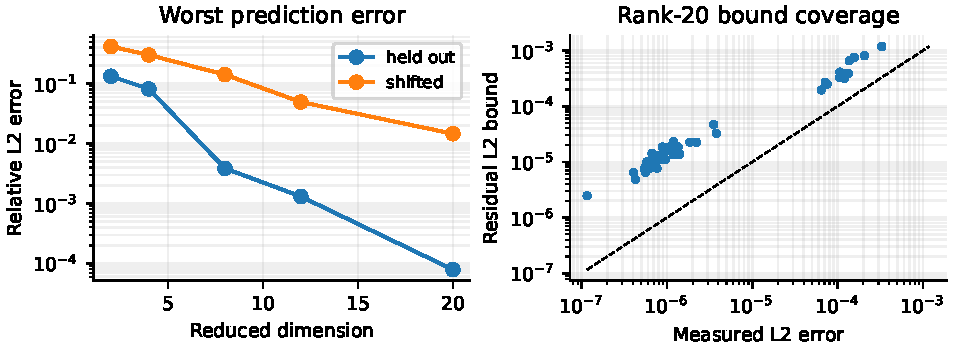
\includegraphics[width=\textwidth]{figure.pdf}
\caption{Recorded worst relative reduction error across ranks and parameter groups (left), and absolute discrete error versus its bound at rank 20 (right). The dashed line denotes equality.}\label{fig:results}\end{figure}
\section{Discussion and limitations}
The held-out error is small for this parameterized family, while the shifted test is materially less accurate. Bound validity does not itself imply that a chosen tolerance has been met: even a low-rank, inaccurate model may pass a coverage check. Coercivity decreases can weaken the bounds, and a small snapshot tail is not an extrapolation guarantee.

The implementation is limited to linear steady conduction on a fixed square with constant coefficients and homogeneous boundary data. It has no transient or nonlinear physics, variable geometry, automatic enrichment, uncertainty quantification, persistence format, or positivity constraint. Extreme scales and ill-conditioned reduced systems are outside the validated regime. Recorded timings are descriptive: fresh full assembly/solve and reduced solve/bounds/output exclude different offline/reconstruction costs, so no general speedup is inferred.
\section{Reproducibility and conclusion}
This note documents the committed implementation at \texttt{098f671c117b} and the existing synthetic results; it does not assert new solver runs. Install from the repository root with \texttt{python -m pip install ".[dev]"}; the README gives compiler requirements and verification commands. Code, data, and this manuscript are available at \href{https://github.com/racostacme-come/podguard}{the project repository}. No private course material is reproduced. The manuscript was prepared with AI assistance under the project owner\textquotesingle s direction; no peer review is claimed.
Run \texttt{podguard --output out --n 39 --rank 20}. Training parameters, singular values, sample audits, spatial convergence, and fields are stored as CSVs with \texttt{validation.json}. The project illustrates a useful separation: compression supplies an approximation, residual estimation assesses it on the discrete model, and a distinct mesh study addresses spatial error.
\begin{thebibliography}{9}
\bibitem{buhr} A. Buhr, C. Engwer, M. Ohlberger, and S. Rave, \emph{A numerically stable a posteriori error estimator for reduced basis approximations of elliptic equations} (2014). \href{https://arxiv.org/abs/1407.8005}{arXiv:1407.8005}.
\bibitem{scipy} SciPy, \emph{scipy.sparse.linalg.spsolve} reference. \href{https://docs.scipy.org/doc/scipy/reference/generated/scipy.sparse.linalg.spsolve.html}{Sparse direct-solve documentation}.
\end{thebibliography}

\end{document}
